%! Author = Ian
%! Date = 11/28/2023

% Preamble
\documentclass{article}

% Packages
\usepackage{amsmath}
\usepackage{fancyhdr}
\usepackage[top=2cm, left=2cm, right=2cm, bottom=2cm]{geometry}
\usepackage{multicol}
\usepackage{amsfonts}
\usepackage{gensymb}
\usepackage{graphics}
\usepackage{graphicx}

\setlength{\columnsep}{0.5cm}

\author{Ian Chen}
\date{\today}

% Header
\fancyhf{}
\fancyhead[L]{Ian Chen}
\fancyhead[C]{CS376 Notes}
\fancyhead[R]{ic8683}
\pagestyle{fancy}

% Document
\begin{document}
    \begin{multicols*}{2}
        \subsubsection*{Structure from Motion}
        \textit{Pinhole Camera}: Test\newline
        \textit{Homogenous Coordinates}: (x, y) $\leftrightarrow$ ($\lambda$x, $\lambda$y, $\lambda$)\newline
        \textit{Intrinsic Parameters}: K-Matrix\newline
        \textit{Extrinsic Parameters}: [R$\mid$t]\newline
        \textit{Projection Matrix}: $\Pi$ = K[R$\mid$t]\newline
        \textit{Essential Matrix}: TR, 5$\degree$ of freedom\newline
        \textit{Epipolar Geometry}: Test\newline
        \subsubsection*{Camera Calibration}
        \textit{Rig}: Test\newline
        \subsubsection*{Stereo Matching}
        \textit{Binocular Stereo}: Test\newline
        \textit{Window Search}: Test\newline
        \textit{Markov Random Field}: Test\newline
        \textit{Graph Cut}: Test\newline
        \subsubsection*{Image Classification}
        \textit{Cross-Validation}: Split training set into n-folds, [0, n-1] for training, [n] for
        testing\newline
        \subsubsection*{KNN}
        \textit{Hyperparameters}: K and Norm(L1 better, reduces background noise)\newline
        \textit{Pros}: Simple\newline
        \textit{Cons}: Expensive(Use PCA), Norm choice\newline
        \textit{Curse of Dimensionality}: Overfitting\newline
        \subsubsection*{Linear Classifier}
        Foundation in neural networks\newline
        \textit{Score Function}: Map data to class scores\newline
        \textit{Loss Function} Quantifies prediction/ground truth disparity\newline
        \subsubsection*{SVM}
        SVM: Hinge loss | Softmax: Cross-entropy loss\newline
        \textit{Multi-Class Loss} Data loss + Regularization loss\newline
        \subsubsection*{Softmax Classifier}
        Provides probabilities for each class\newline
        \textit{Cross-Entropy Loss}: Maximize cross-entropy\newline
        \subsubsection*{AdaBoost}
        Ensemble method, combine weak(base) learners to form strong learner, robust to
        overfitting\newline
        \textit{Weak Learner}: Error$<$50\%\newline
        \subsubsection*{Viola-Jones Face Detector}
        Uses AdaBoost\newline
        \textit{Haar-like Features}: +/- Rectangles\newline
        \textit{Integral Image}: II$_{ij}$ = $\sum$i$_{x\leq i;y \leq j}$ \newline
        \textit{Classifier Cascade}: Each successive strong classifier uses more features, lower
        threshold to reduce false negative(increase false positive), Every classifier must be
        positive to be classified as positive\newline
        \subsubsection*{Neural Network}
        Layers of neurons, each neuron is a linear classifier, each layer is a non-linear transformation\newline
        \textit{Score Function}: Employs activation function\newline
        \textit{Activation Function}: Non-Linear\newline
        \subsubsection*{Pooling Layer}
        Downsamples spatial dimensions, reduces computation\newline
        \textit{Max Pooling}: Take max of each window to downsample\newline
        \subsubsection*{Fully-Connected Layer}:
        \textit{Neurons} Connected to every neuron of next layer\newline
        \subsubsection*{Convolutional Layer}
        Colloquially uses cross-correlation, uses CONV/FC/POOL layers\newline
        \textit{Output Size(Image$_{N\times N}$, Filter$_{F \times F}$)}: (N - F)/(stride + 1)\newline
        \textit{Stride}: Jump of filter over image\newline
        \textit{Padding}: To make output same size\newline
        \textit{Hyperparameters}: \# filters, filter size, stride, padding\newline
        \subsubsection*{Gradient Descent}
        \textit{Numerical}: Slow, Approximate, Easy to Write\newline
        \textit{Analytic}: Fast, Exact, Error Prone\newline
        \subsubsection*{Backpropagation}
        \textit{Forward/Backward API}: Forward- Compute operations, save immediates for gradient
        computation, Backward- Apple chain rule to compute gradient of loss function\newline
        \subsubsection*{Object Detection}
        \textit{Window-Based}: Viola-Jones, Stengths- Simple detection protocol, good feature
        choices critical, past successes for certain classes, Flaws- High computational
        complexity, need low false positive rates, not all objects box shaped, assumes fixed
        viewpoint\newline
        \subsubsection*{Object Proposals}
        \textit{Proposals}: Object-like regions\newline
        \textit{Person Detection}: HoG and linear SVM\newline
        \textit{Dalal-Triggs Method}: Sliding Window, HoG, + linear SVM\newline
        \textit{Deformable Part Model}: Star Model- Coarse Root Filter + Higher resolution part
        filters\newline
        \textit{Object Hypothesis}: Level+Position of the i-th filter\newline
        \subsubsection*{Active Contour}
        \textit{Test}: Test\newline
        \subsubsection*{R-CNN}
        Pre-trained, fine-tuned on PASCAL VOC\newline
        \subsubsection*{Decision Tree}
        Testing attribute should split training samples into subsets that are as pure as possible\newline
        \textit{Leaves}: Decisions\newline
        \textit{Information}: Reduction in uncertainty\newline
        \textit{Entropy}: Expected amount of information\newline
        \textit{Information Gain}: Information before split - after\newline
        \textit{Bagging}: Reduce variance, committee of trees, samples with replacement\newline
        \textit{Random Forest Classifier}: ex. Microsoft Kinect, efficient, distributed,
        variable importance, easy to update algorithm, cons: interpretability\newline
        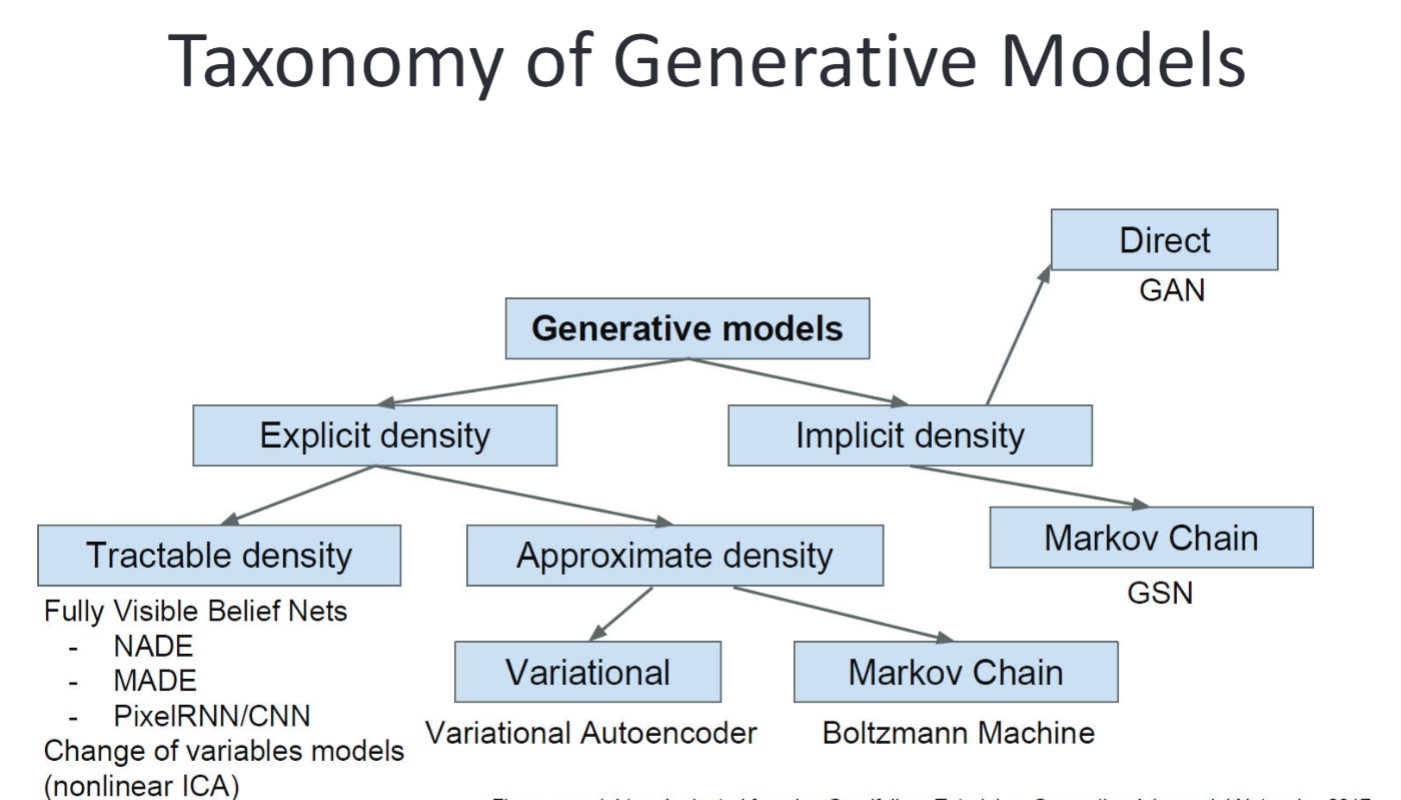
\includegraphics[width=0.5\textwidth]{generative_models}\newline
        \subsubsection*{Generative Models}
        \textit{Generative Adversarial Networks}: Test\newline
        \textit{Variational Autoencoder}: Autoencoder- Reconstruct data\newline
        \subsubsection*{Semantic Segmentation}
        \textit{Markov Random Field}: Smooth\newline
        \textit{Sliding Window}: Approach 1\newline
        \textit{Fully Convolutional}: Approach 2\newline
        \subsubsection*{Instance Segmentation}
        \textit{FCN Methods}: Divide results from semantic segmentation into individual instances\newline
        \textit{RCNN Methods}: Use segmentation level proposals then train classifier to classify
        proposals\newline
    \end{multicols*}
\end{document}